\documentclass{article}
\usepackage[T1]{fontenc}
\usepackage{lmodern}
\usepackage{graphicx}
\usepackage{amsmath,amssymb}
\usepackage[a4paper,margin=2cm]{geometry}
\usepackage[absolute,overlay]{textpos}
\setlength{\TPHorizModule}{1mm}
\setlength{\TPVertModule}{1mm}
\usepackage[indonesian]{babel}
\usepackage{hyperref}
\setlength{\emergencystretch}{2em}
% unit: Halaman 6

\begin{document}

% === Halaman 6 (llm) ===

\vspace{216.81mm}

\begin{itemize}
    \item $\text{GOST menggunakan Jaringan Feistel}$
    \item $\text{Satu putaran GOST:}$
    \[
    \begin{aligned}
    L_i &= R_{i-1} \\
    R_i &= L_{i-1} \oplus f(R_{i-1}, K_i)
    \end{aligned}
    \]
    \vspace{60mm}
    \item $\text{Fungsi } f \text{ terdiri dari}$
    \begin{itemize}
        \item $\text{penjumlahan dalam modulus } 2^{32}$
        \item $\text{substitusi}$
        \item $\text{pergeseran}$
    \end{itemize}
\end{itemize}

\vspace{20mm}
\noindent Keterangan: $\boxed{\begin{smallmatrix} \square \end{smallmatrix}}$ adalah operator penjumlahan dalam modulo $2^{32}$

% deskripsi: Diagram alir struktur Jaringan Feistel untuk satu putaran algoritma GOST, menunjukkan aliran data L dan R, fungsi f dengan substitusi S-Box dan pergeseran sirkuler, serta operasi XOR.
% bbox normalisasi: [0.5500, 0.1400, 0.9400, 0.8700]
\begin{textblock*}{81.90mm}(115.50mm,41.58mm)
\noindent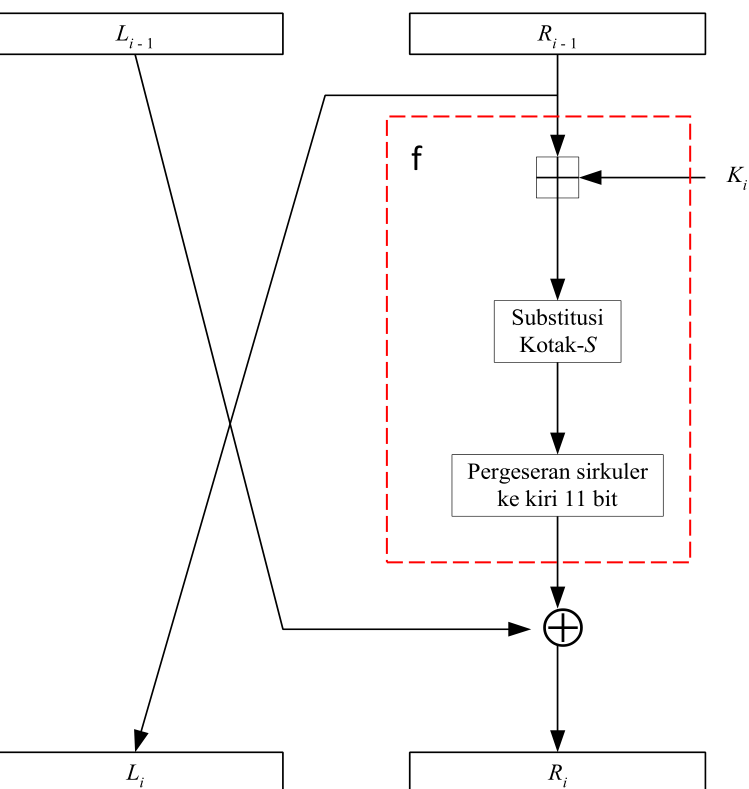
\includegraphics[width=81.90mm,height=216.81mm]{../../images/llm/page_006_img_01.png}%
\end{textblock*}

\end{document}
